\chapter{Evaluation} \label{chap:evaluation} \minitoc

\section*{}

This section evaluates how the solution developed proves the hypothesis proposed in Chapter \ref{chap:problem_statement}.

\textcolor{blue}{Complete...}

% First, an explanation of the scenarios will be made, as well as their relation to the features developed and their advantages. 

\section{Scenarios and Experiments}\label{sec:scenarios_experiments}

The testing of the proposed solution diverged in two different scenarios. The first simulates physical devices with the use of Docker containers running the Unix port of MicroPython, allowing the construction of scalable scenarios with minimal costs. The second scenario uses physical devices, such as ESP8266 and ESP32, connected to the same Wi-Fi.

\begin{enumerate}
    \item A room has 3 sensors that give temperature and humidity readings every minute. There’s a virtual sensor that compares the results (of both temperature and humidity) and triggers depending on some configured thresholds. An AC uses those readings to decide (a) if it switches on/off, (b) its operating mode: cool, heat, and dehumidify. The Minimal Working System (MWS) consists in (a) one temperature sensor, (b) one humidity sensor, (c) one node capable of making the decision, and (d) working communication channels amongst them.
    \item 20 devices, where each device redirects its input to its output. \textcolor{red}{improve}
\end{enumerate}

The first scenario aims to test the features of the developed solution with a moderately simple Node-RED flow, taking advantage of the nodes developed for MicroPython code generation support. The second scenario allows the comparison of the developed solution to the already existing solutions.

\textcolor{red}{Refactor this enumeration, with some explaining of some terms}

\textbf{Scenario 1}:
\begin{enumerate}
    \item \textbf{Sanity check.} All tasks are simple readings and forwarding, no compensation or other fault-tolerance strategy. Each sensor does its own thing. Orchestration is centralized. We expect all roundtrips to take less than the smallest part that can be resolved (measurement capability, which we estimate to be <1s). This will be executed using both Docker containers and physical devices.
    \item \textbf{Re-orchestration.}
        \begin{itemize}
            \item \textbf{Experiment A.} MWS is achieved via multiple possible configurations by selective (provoked) device failure (fail-stop);
            \item \textbf{Experiment B.} Inconsistent device behaviour, e.g. appear and disappear in shorter intervals lower that the time needed for orchestrating convergence (OCT), that leads to activity impacting the MWS;
            \item \textbf{Experiment C.} With 4 devices, each one with different processing capabilities. During orchestration, some devices will develop an out-of-memory error because they can't process all the processing tasks assigned to them, specifically the size of the script given. The orchestrator decides to send less tasks to these devices. The system will converge in a working solution. \textit{This scenario will be implemented with a modified device script. When devices receive a script, it will generate a memory error if the length of the script passes a certain threshold. This simulates the memory constraints of devices when receiving a file to big.}
            \item \textbf{Experiment D.} With 4 devices, some of them have a memory leak with an unknown cause. After random time Random(t0,t1), these problematic devices stop working with an out-of-memory error. The orchestrator thinks that the devices can't handle the quantity of processing tasks assigned to them, so in the re-orchestration it will assign fewer tasks. Since these devices will always break, the orchestrator will eventually not consider these devices in the assignment of nodes. \textit{This scenario will be implemented with a modified device script that will trigger an out-of-memory error after a random period after executing the given tasks.}
            \item \textbf{Experiment E.} With 4 devices, there is a device that is sensitive to a particular node, which causes the device to give out an out-of-memory error. The orchestrator will potentially assign this node to the specific device. When the device gives out the out-of-memory error, the orchestrator will eventually converge in a solution where the node is not assigned to the particular device, and the system will converge.  \textit{These out-of-memory errors will be simulated with the use of a failure node that forces an \texttt{MemoryException} in the device.}
            \item \textbf{Experiment F.} With 50 devices, each second the device has a probability to fail. This failure can go from 0 to 10 seconds, randomly chosen. The orchestrator must deal with the random failure of the devices and re-orchestrate the system. This experiment is considered a stress test, causing repeated failures and forcing constant re-orchestration.
        \end{itemize}
        Verifies that:
        \begin{enumerate}
            \item \textbf{Restrictions (predicates) are enforced.} Check that possible configurations lead to solutions that enforce defined predicates;
                \begin{enumerate}
                    \item Temperature and humidity might coexist in the same, or in dedicated, devices;
                \end{enumerate}
            \item \textbf{Priorities are honored.} Check that all specified priorities were taken into account, and only violated if necessary;
                \begin{enumerate}
                    \item Priority is given to edge devices, but fog and cloud can be used;
                    \item Priority is given to the maximum level of decentralization, but some centralization can be used.
                \end{enumerate}
        \end{enumerate}
\end{enumerate}

\textbf{Scenario 2}:
With the use of 20 physical devices, both ESP8266 and ESP32, implement a line topology, where a message is sent to a starting device, that will propagate it to its output. All the devices implement this propagation logic, which results in the initial message reaching the end of the line. The propagation time is measured, starting when the message is sent and ending when the message reaches the last node.
This experience is implemented in several environments:
\begin{enumerate}
    \item \textbf{Node-RED original}. Runs the experiment in the original Node-RED, using the default option (events) as the communication channel between nodes.
    \item \textbf{Node-RED + MQTT}. Run the experiment in Node-RED, using MQTT as the communication channel between nodes.
    \item \textbf{Node-RED modified + Dockers (same host)} Runs the experiment in the modified version of Node-RED, with each node assigned to a different virtual device, running in a Docker container. The Docker containers are running the firmware created in a Unix MicroPython port. The virtual devices are in the same host machine running the MQTT server instance.
    \item \textbf{Node-RED modified + Dockers (different host)} Runs the experiment in the modified version of Node-RED, with each node assigned to a different virtual device, running in a Docker container. The Docker containers are running the firmware created in a Unix MicroPython port. The MQTT server instance is in a different host machine from the one running the virtual devices. All machines are connected through Wi-Fi.
    \item \textbf{Physical + MQTT} Runs the experiment in physical devices without the developed firmware. Each device runs a simple MicroPython script that executes the wanted behaviour, communicating by MQTT. No Node-RED is used.
    \item \textbf{Node-RED modified + MQTT + Physical + Firmware} Runs the experiment with the developed solution, with each node assigned to a different physical device running the developed MicroPython firmware. All communicating is made using MQTT.
\end{enumerate}

\section{Discussion}\label{sec:evaluation_discussion}

\textcolor{blue}{Complete...}

\subsection{Scenario 1}\label{sec:discussion_scenario1}

As mentioned previously, the first scenario consists of a system that controls an A/C. This system takes into account readings of 3 temperature and humidity sensors to define if the room's temperature is too hot, cold of humid and sends commands to the A/C with the respective actions. The Node-RED implementation of this system can be seen in Figure \ref{fig:scenario1_node_red}.

\begin{figure}[h]
\centering
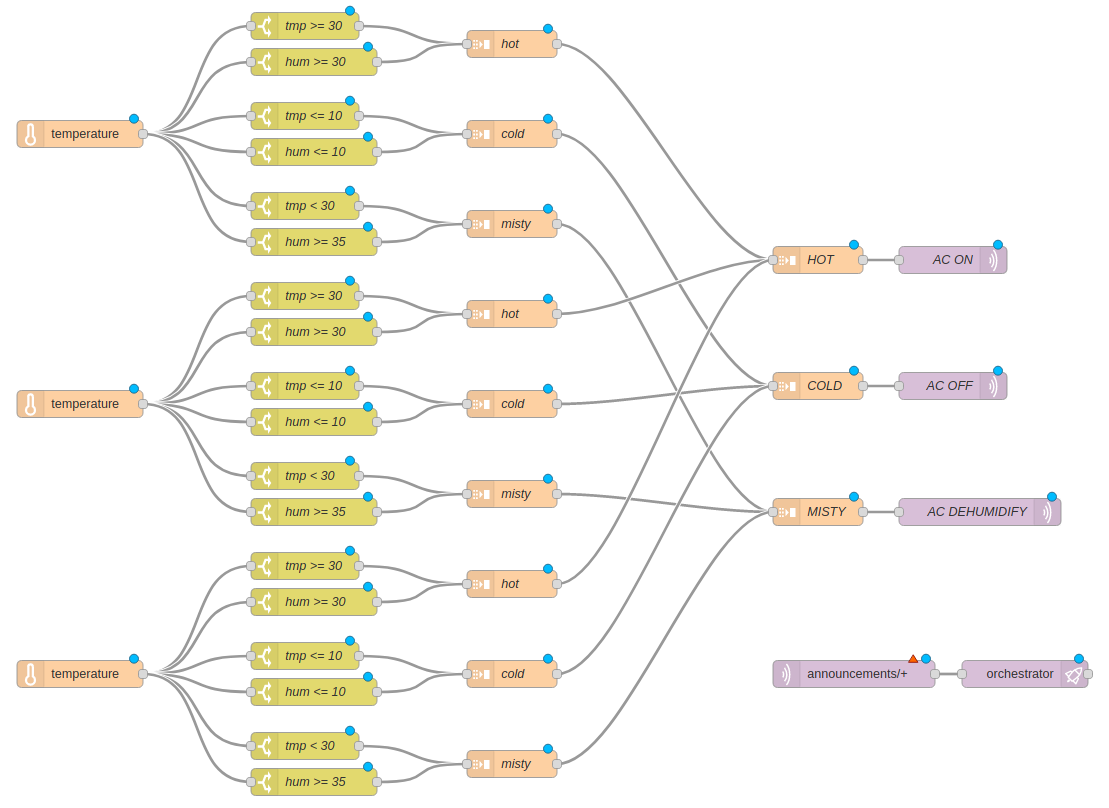
\includegraphics[width=\textwidth]{scenario1.png}
\caption[Node-RED implementation of scenario 1]{Node-RED implementation of scenario 1}\label{fig:scenario1_node_red}
\end{figure}

The sanity check experiments will prove that the devices can satisfy the nodes, meaning that the system works as its meant to once the assignment is completed. With this premise, this will not verified in the other experiments.

%%%%%%%%%%%%%%%%%%%%%% SC %%%%%%%%%%%%%%%%%%%%%%

\subsubsection{Sanity Check}\label{sec:sanity_check_exp}

The first experiment made to the developed solution tested the overall functionality of the tool and its efficiency. Using 4 Docker containers with the MicroPython Unix port with the developed firmware, the scenario presented in Figure \ref{fig:scenario1_node_red} was partitioned and assigned evenly to them. The assignment can be observed in Figure \ref{fig:sanity_check_graph}, where it was allocated 9 \textit{nodes} for each device.

\begin{figure}[h]
\centering
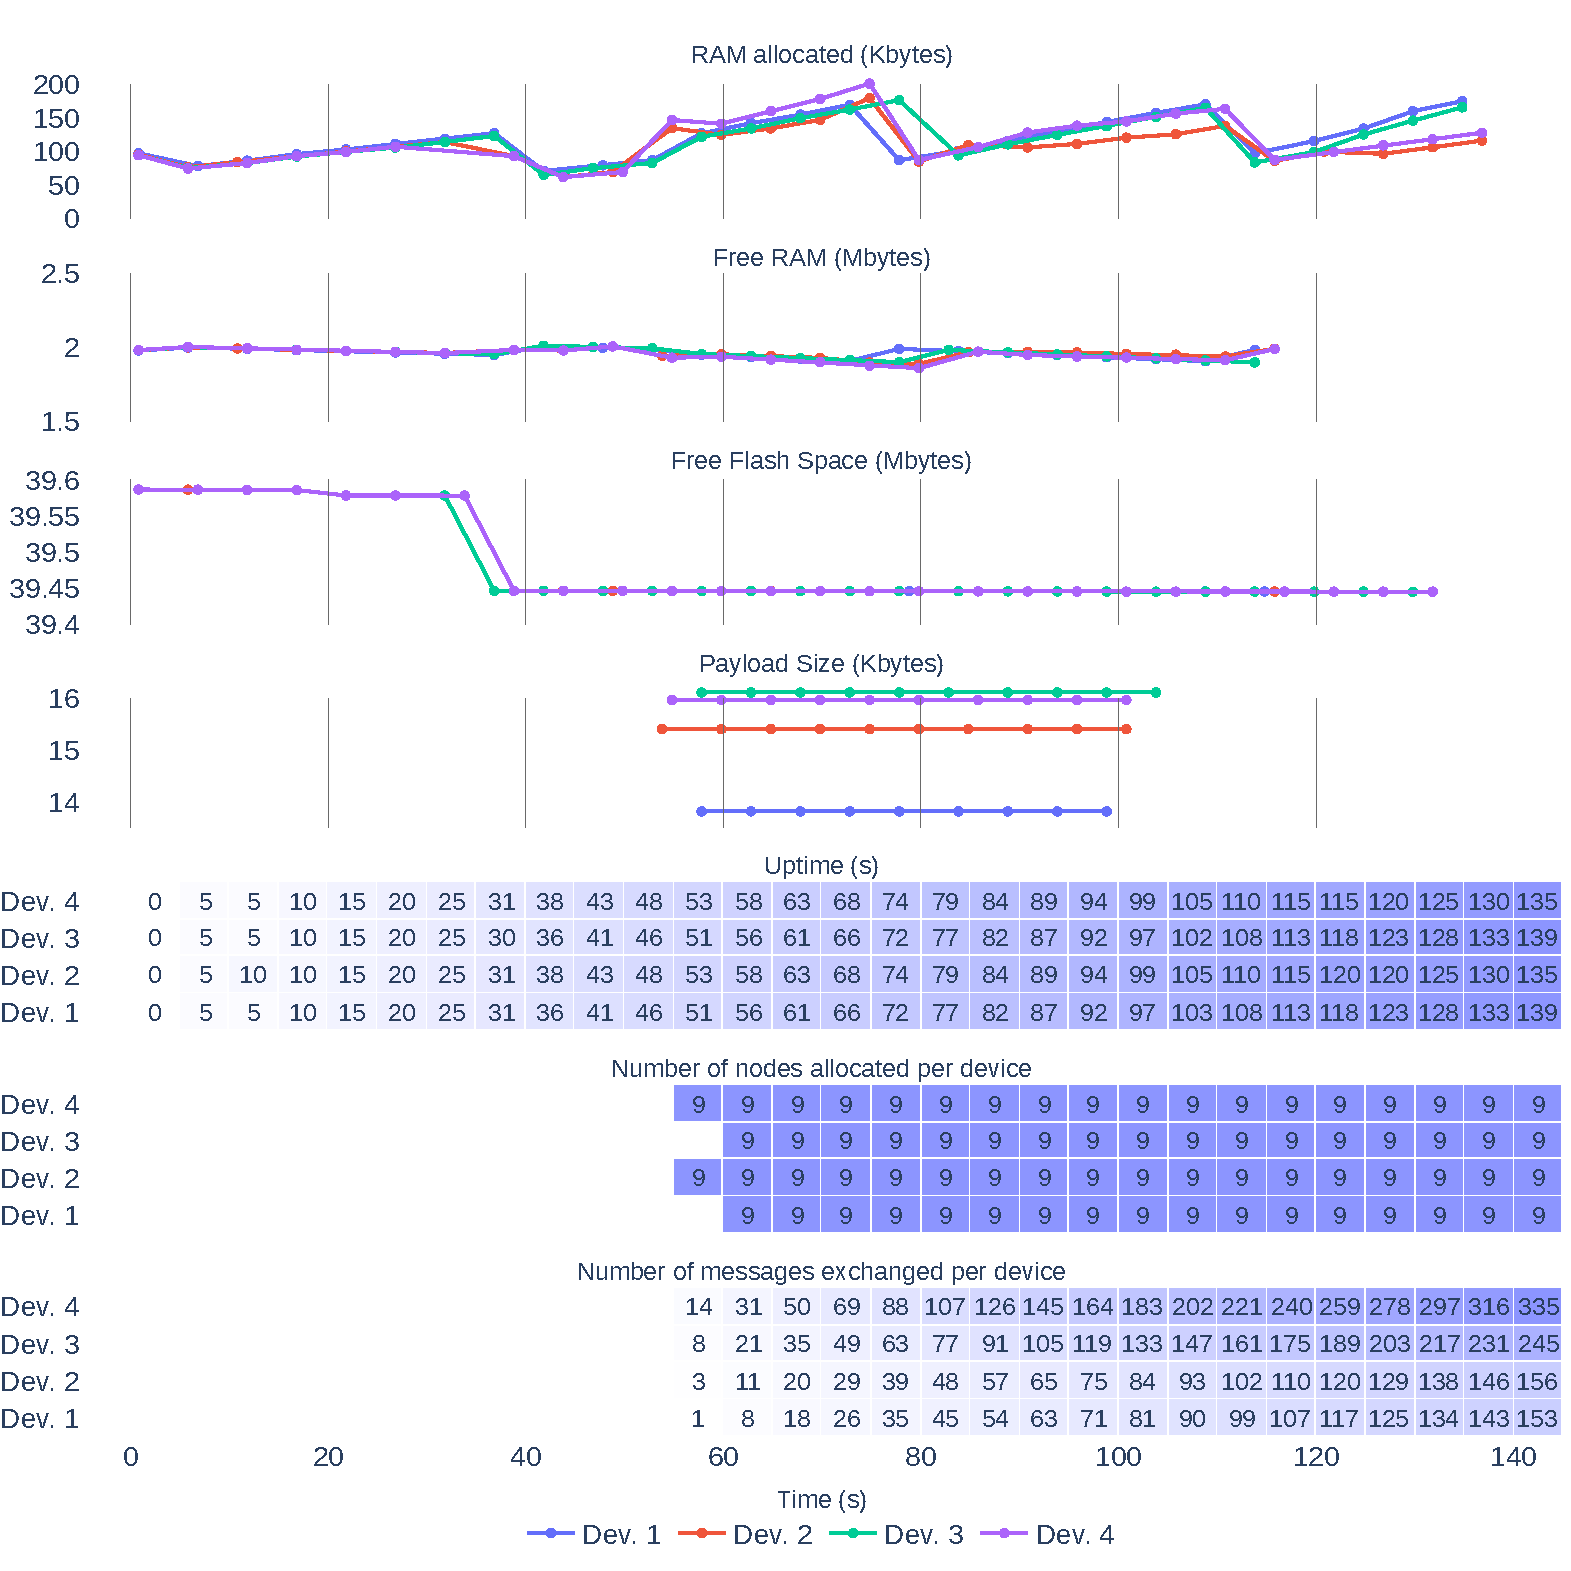
\includegraphics[width=\linewidth]{experiences/1-sanity_check/sanity_check.pdf}
\caption[Sanity check experience measurements]{Sanity check experience measurements}\label{fig:sanity_check_graph}
\end{figure}

The usage of RAM was significant, varying from 60Kb to 200Kb, as it can be observed in Figure \ref{fig:sanity_check_graph}. The flash size only decreases around 150000 bytes, when the device receives a script to execute. This quantity matches the overall payload received by the devices.

As mentioned before, once the orchestrator defines the \textit{nodes} assignment, a script is built and send to the devices. The confirmation of this delivery is necessary for the system to conclude the assignment phase and start the constant verification of the state of the system. The time it takes to deliver the script was timed and it can be consulted in Figure \ref{fig:sanity_check_graph}. The usage of virtual devices running in the same host as the Node-RED instance allows for smaller times, which are measured in milliseconds.

Once the devices execute the script given to them, each \textit{node} allocated to a device start to communicate with each other, publishing and consuming MQTT messages. To verify that the system works, the messages of all communicating topics were captured. This messages prove that the system works, since all \textit{nodes} are receiving their inputs and producing outputs. The number of communications can be consulted in Figure \ref{fig:sanity_check_graph}. As it can be observed, the number of communications in Device 1 is bigger than any other. This is due to the fact that in this device two temperature-humidity \textit{nodes} were allocated, which publish 3 messages, a number communication events bigger than any other node. The Device 2 contains the other temperature-humidity node.

It can be concluded from this sanity check experiment that the solution developed works, not only by spreading the computation throughout the available devices, but it also results in a functional system.

\textcolor{red}{Include \textit{node} assignment of nodes? JSON? Or modify the node-red flow and say the device each \textit{node} was assigned to?}

\todo[inline]{Is it necessary to add the table/graph with the times it took to send the scripts to the devices?}

%%%%%%%%%%%%%%%%%%%%%% SC Phys %%%%%%%%%%%%%%%%%%%%%%

\subsubsection{Sanity Check with Physical Devices}\label{sec:sanity_check_phys_exp}

The sanity check experiment was repeated using physical devices, more specifically 4 ESP32. Similar to the virtual devices, the assignment of \textit{nodes} to devices spread the number of \textit{nodes} equally, with each device having 9 \textit{nodes} to their responsibility. This assignment result can be seen in Figure \ref{fig:sanity_check_phys_graph}.

\begin{figure}[h]
\centering
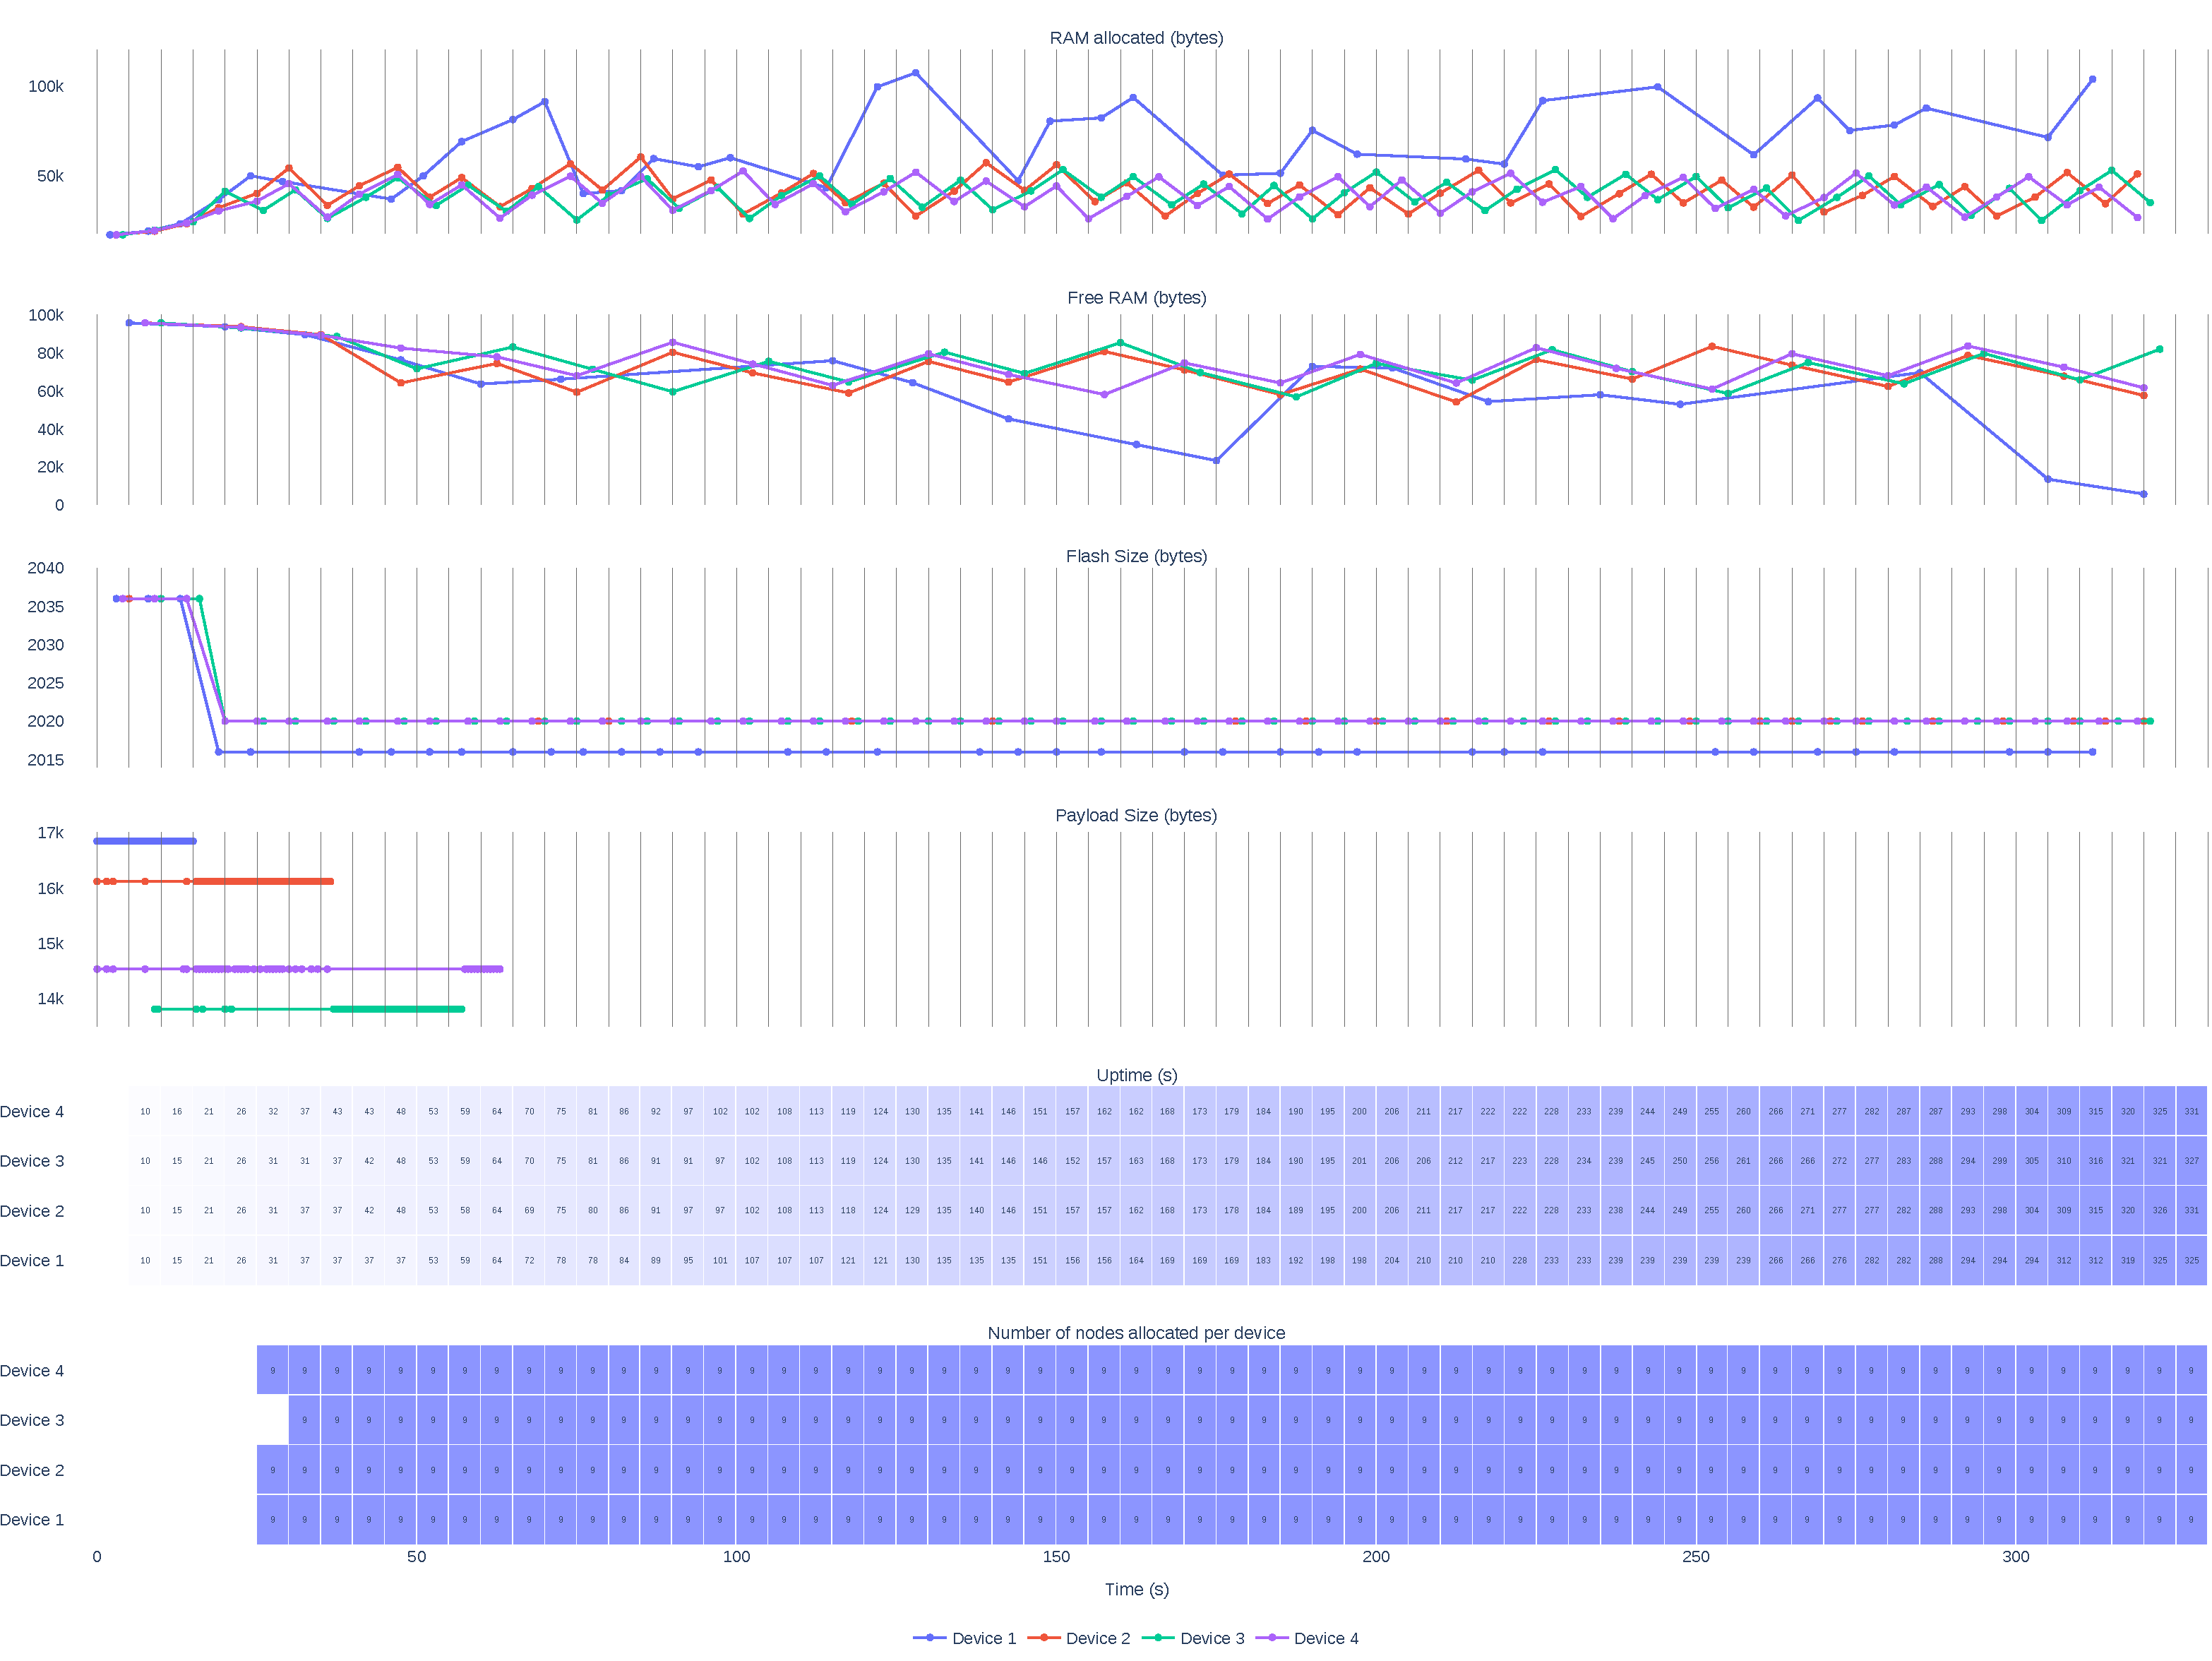
\includegraphics[width=\linewidth]{experiences/1-sanity_check_phys/sanity_check_hardware.pdf}
\caption[Sanity check with physical devices experience measurements]{Sanity check with physical devices experience measurements}\label{fig:sanity_check_phys_graph}
\end{figure}

The usage of RAM in physical devices is smaller than the one used by virtual devices. This can be explained with the possible optimization differences in the MicroPython ports, as well as the changes implemented in libraries to support the Unix port.

The flash size of the physical devices is smaller than the physical ones, as expected. It can be observed in Figure \ref{fig:sanity_check_phys_graph} that the device with the biggest payload, Device 1, ends up having the smaller flash size, which is logical. The overall size of the payloads are very similar to the ones in the previous experiment. 

The script delivery time for physical devices is bigger than the virtual devices. Since they are not running in the same machine, the WiFi stack as well as the devices' hardware hinder the speed of communication. The uptime is similar to the previous experiment, since no device failed.

%%%%%%%%%%%%%%%%%%%%%% Exp A %%%%%%%%%%%%%%%%%%%%%%

\subsubsection{Experiment A}\label{sec:exp_a}

This experiment aims to test the system's ability to re-orchestrate when a device fails or becomes available. During the occurrence of the experiment, devices were turned off one by one until only one was left running. The expected behaviour is that the system detects that a device has become unavailable and re-orchestrates, assigning \textit{nodes} to the available devices. In the end, only one device is running and all the \textit{nodes} are assigned to it.

It can be observed in Figure \ref{fig:experiment_a_graph} that the uptime of the devices stops increasing one by one, identifying the moment the device fails. Once a failure happens, the system (re)orchestrates, assigning the nodes of the device to the other available devices, increasing their number. This can also be observed in Figure \ref{fig:experiment_a_graph}. This increase in the number of nodes assigned to the available devices can also be observed in the payload size. When all devices fail except one, the one remaining is the only one that receives the payload, which is higher than any other previously received.

The information regarding the number of nodes is not updated to 0 once the device fails, since it is no longer active to send the updated metric. 

This experiment proves that the system identifies the failure of devices and takes actions to rectify it. This includes repeating the assignment process, taking into account the available devices.

\begin{figure}[h]
\centering
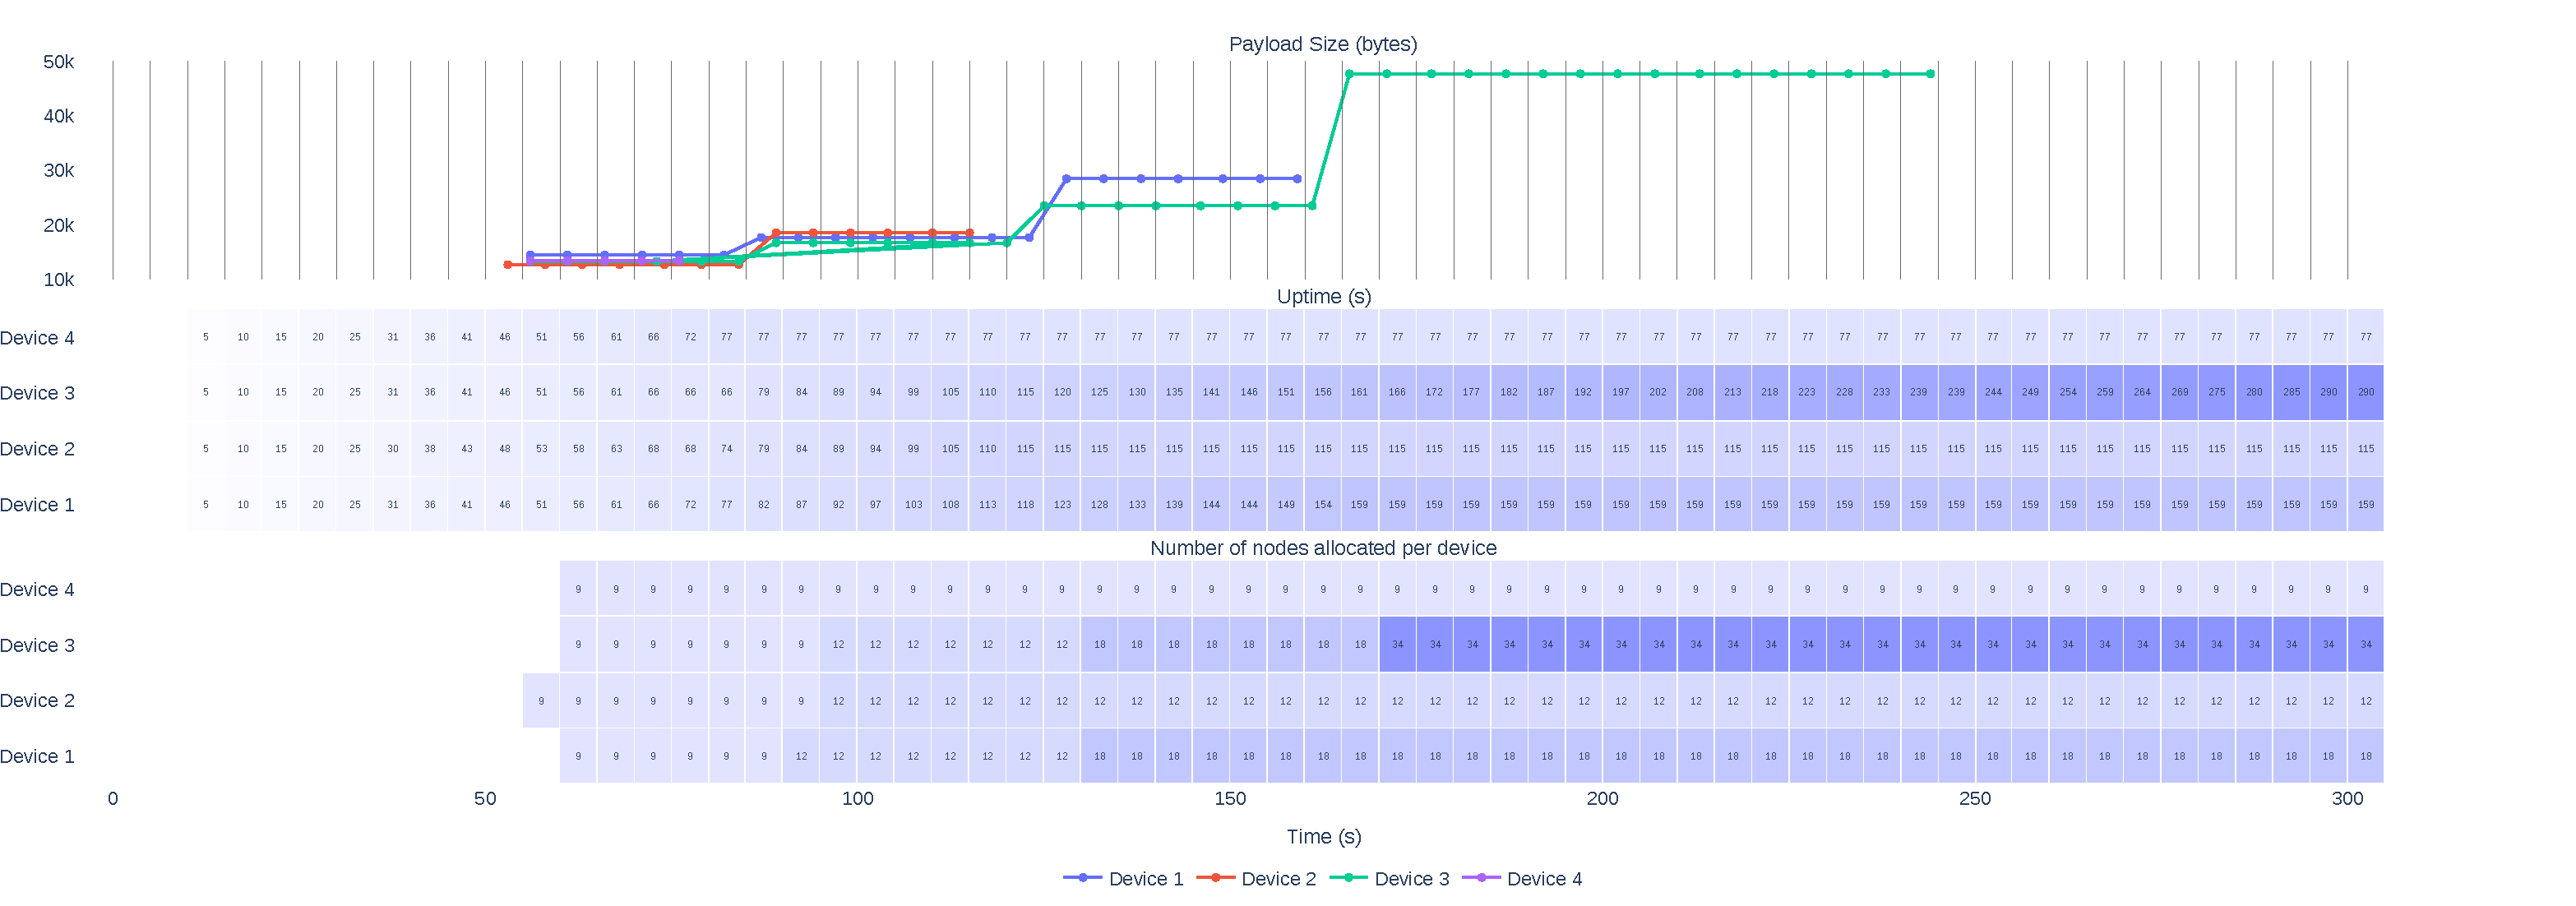
\includegraphics[width=\linewidth]{experiences/A-reorchestration/reorchestration.pdf}
\caption[Experiment A measurements]{Experiment A measurements}\label{fig:experiment_a_graph}
\end{figure}

%%%%%%%%%%%%%%%%%%%%%% Exp A Phys %%%%%%%%%%%%%%%%%%%%%%

\subsubsection{Experiment A with physical devices}

This experiment is very similar to the previous one, the only difference is in the use of physical devices instead of virtual ones. The payloads and number of nodes assigned through the experiment is very similar to the ones achieved with virtual devices. The only thing to note is the fact that Device 2, the  last remaining active device, fails when receiving the bigger payload. This payload contains the code for all the nodes of the system, since no other device is available. 

This exposes one of the limitations of using physical devices, the memory. The device does not have enough memory to handle that big of a script, so it \textsc{fail-safe}s, informing the system that there was an \textit{Out-of-Memory} error. In its turn, the system assigns less nodes to the device.

\begin{figure}[h]
\centering
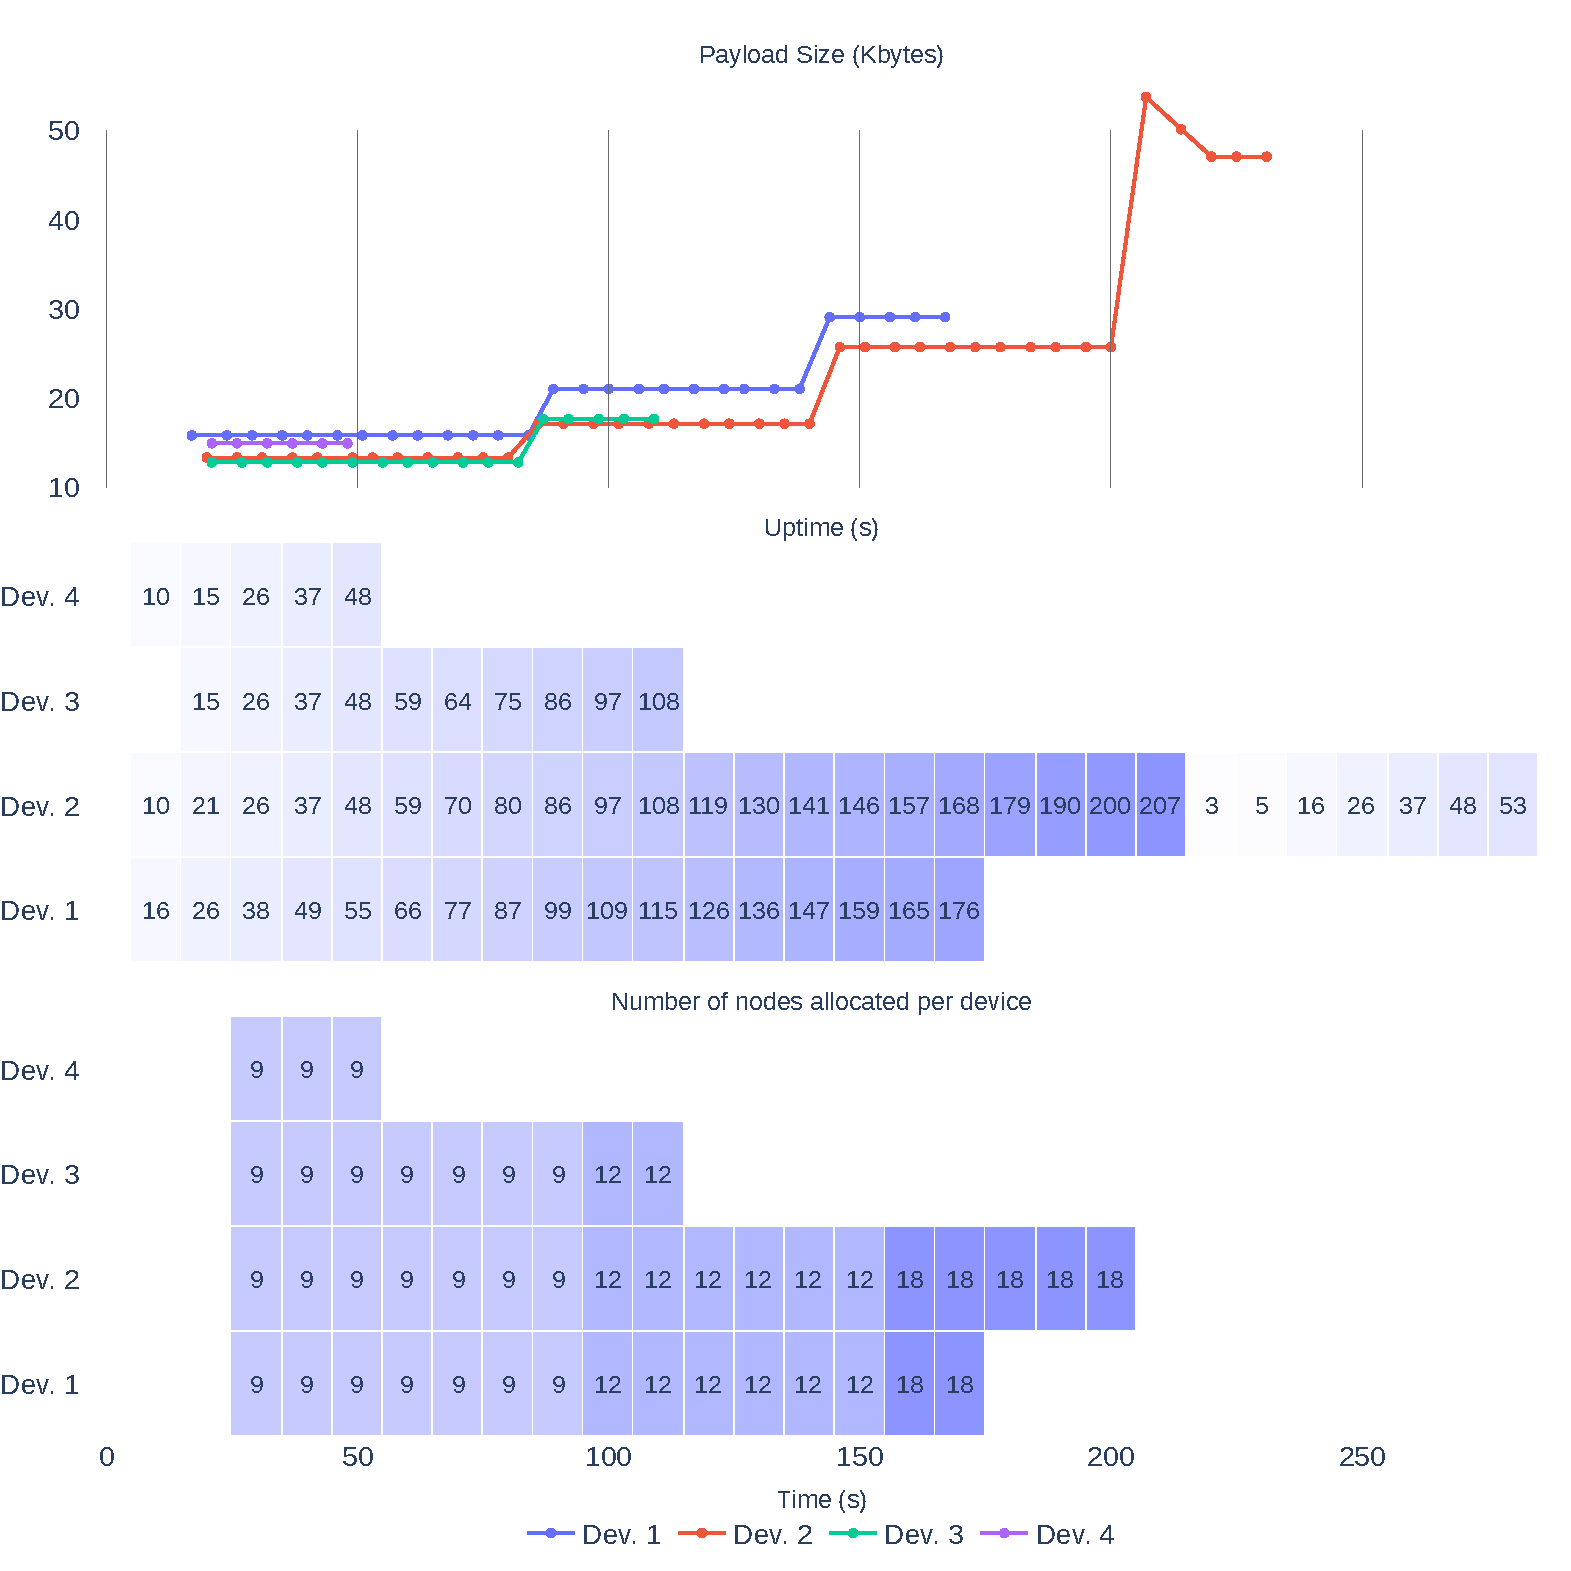
\includegraphics[width=\linewidth]{experiences/A-reorchestration_phys/reorchestration_phys.pdf}
\caption[Experiment A with physical devices measurements]{Experiment A with physical devices measurements}\label{fig:experiment_a_phys_graph}
\end{figure}

%%%%%%%%%%%%%%%%%%%%%% Exp B %%%%%%%%%%%%%%%%%%%%%%

\subsubsection{Experiment B}

Similar to the two previous experiments, this one takes it a step further, not only testing the system's ability to recover when devices fail, but also when they recover. In Figure \ref{fig:experiment_b_graph}, Device 3 and 4 fail early on and the system recovers, spreading the nodes assigned to them to other devices. Device 4 recovers around the 100s, fails again and then recovers. This change was not caught by the system, since it was very fast, and the system only re(orchestrates) the second time Device 4 recovers. During the course of the experiment, Device 3 and 4 continue to fail and recover, and the system always adapts.

This ability for the system to re(orchestrate) when a device recovers can be taxing to the functionality of the system. If a device is constantly failing and recovering, the system will always adapts itself, halting its functionality to orchestrate itself.

\begin{figure}[h]
\centering
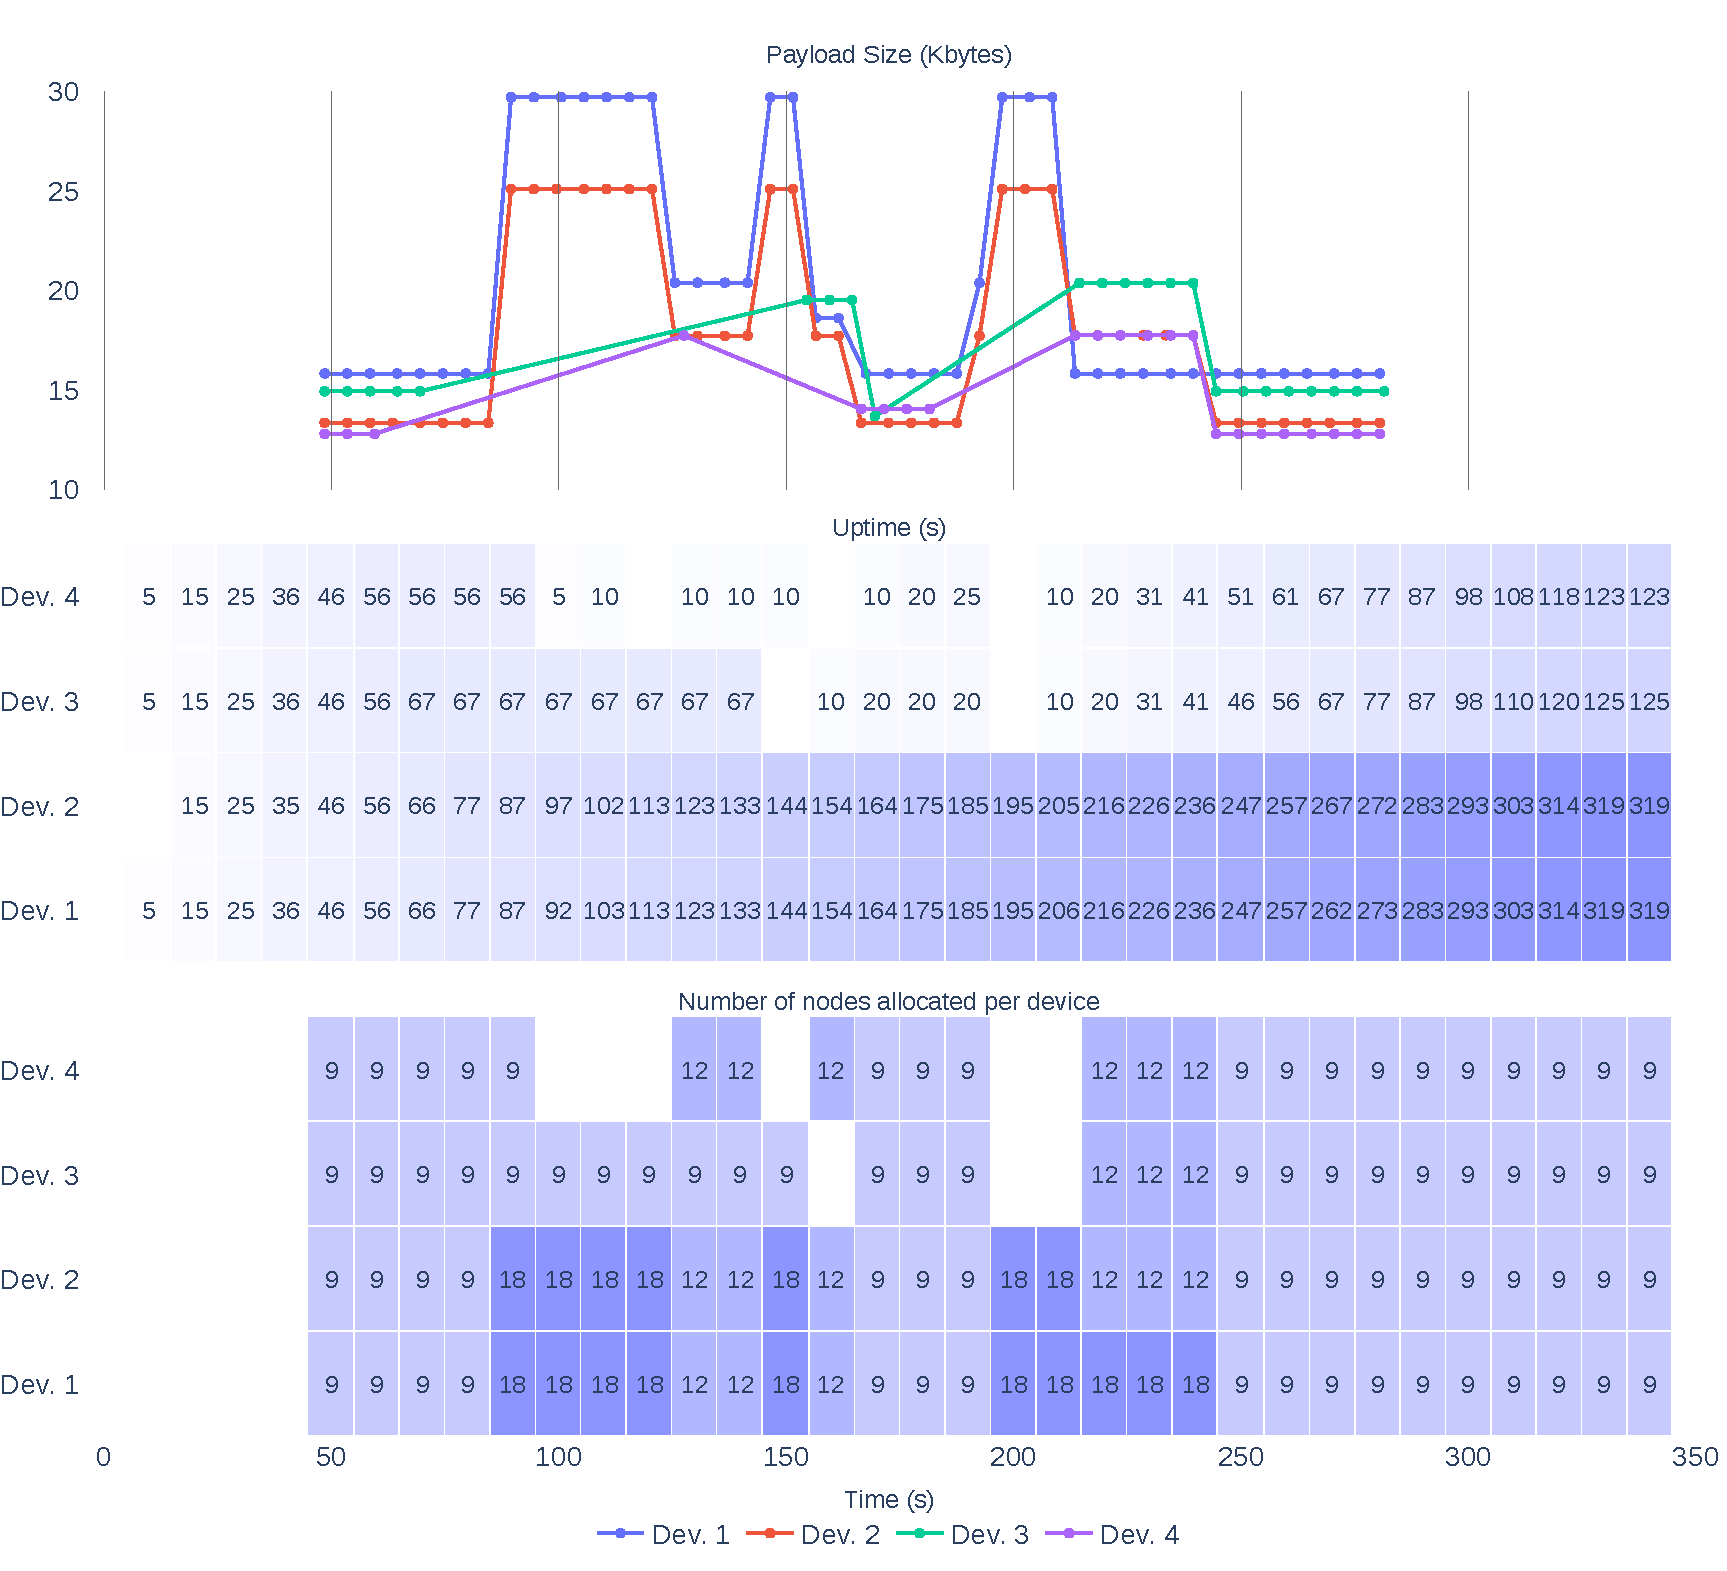
\includegraphics[width=\linewidth]{experiences/B-reorchestration-inconsistent/reorchestration_inc.pdf}
\caption[Experiment B measurements]{Experiment B measurements}\label{fig:experiment_b_graph}
\end{figure}

%%%%%%%%%%%%%%%%%%%%%% Exp C %%%%%%%%%%%%%%%%%%%%%%

\subsubsection{Experiment C}

This experiment aims to test the system's ability to recover and adapt to the devices' memory constraints. More specifically, memory errors that can arise when writing the received script into the device SPI.

In the Figure \ref{fig:experiment_c_graph}, both the Device 2 and 4 are memory constrained. When the first assignment is made, around the 50 seconds, both these devices \textsc{fail-safe} due to \textit{Out-of-Memory} errors. The number of nodes presented in Figure \ref{fig:experiment_c_graph} are the ones assigned after devices 2 and 4 communicate to the orchestrator their limitations. 

To assess if the system saves information about the limitations of the devices, one of them was turned of and later turned on. This event is identified in the Figure \ref{fig:experiment_c_graph}. As it can be observed, Device 2 uptime stops increasing around the time of the event and its nodes are distributed by the other devices, with the exception of Device 4, which is memory constrained. 
After the recovery of Device 2, the system (re)orchestrates and the same number of nodes is assigned to the devices. However, Device 4 failed when Device 2 recovered. This implies that the system repeated the process assignment process again, ignoring the previously known information about memory constraints.

\begin{figure}[h]
\centering
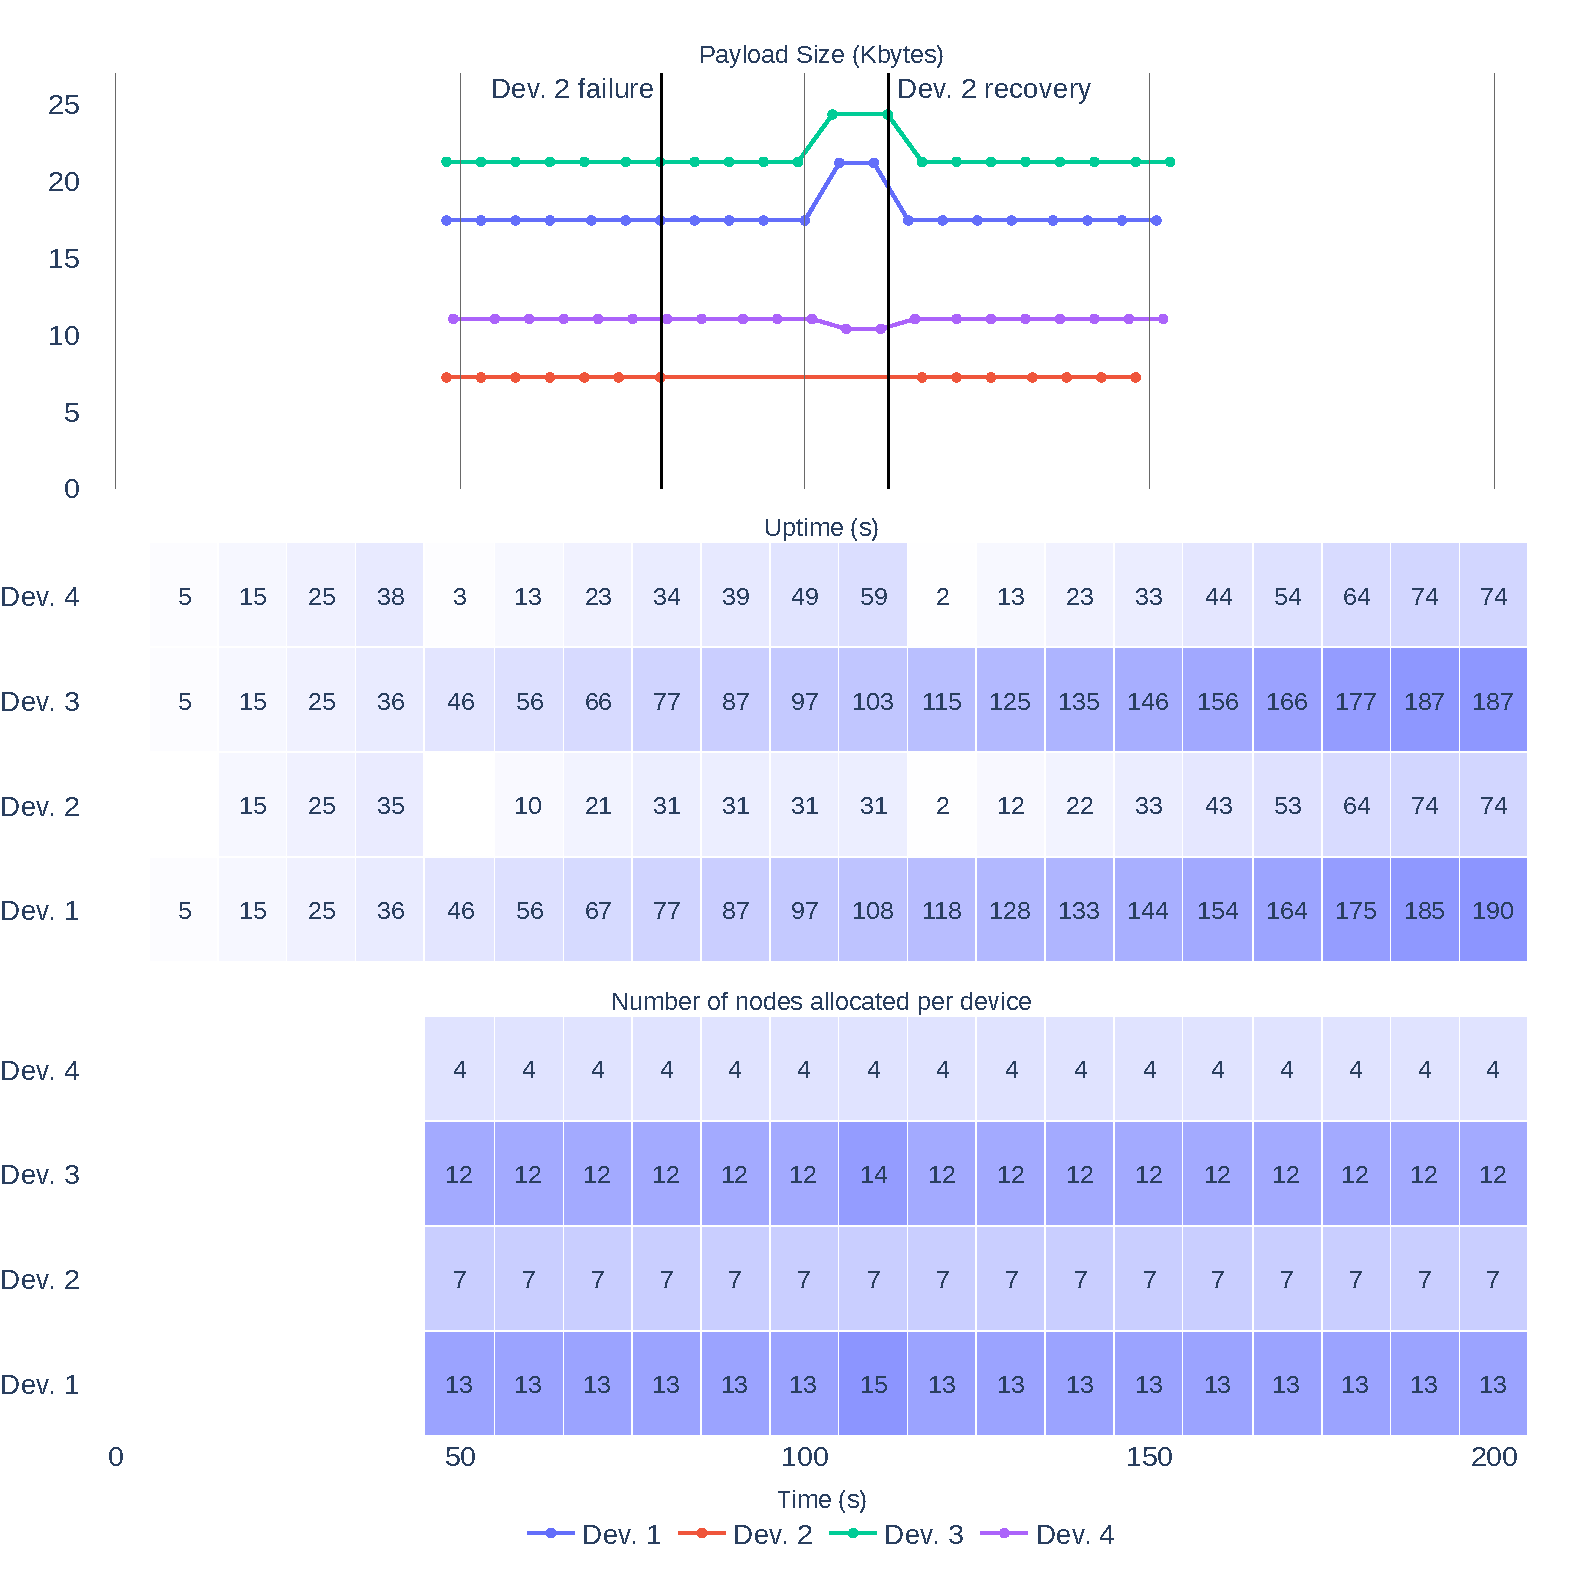
\includegraphics[width=\linewidth]{experiences/C-memory_error_on_write/memory_write.pdf}
\caption[Experiment C measurements]{Experiment C measurements}\label{fig:experiment_c_graph}
\end{figure}

%%%%%%%%%%%%%%%%%%%%%% Exp D %%%%%%%%%%%%%%%%%%%%%%

\subsubsection{Experiment D}

In this experiment the goal is to check into the system's ability to handle a damaged device that has a memory leak. This device, which in this situation is Device 2, will always generate an \textit{Out-of-Memory} error after a random period of time. The system should be able to exclude this device during the course of the assignment process.

As it can be observed in Figure \ref{fig:experiment_d_graph}, Device 2 is consistently failing after the first assignment of nodes, around 75 seconds. The number of nodes assigned decreases, until no node is assigned and the device is excluded from consideration. This is an iterative process, in which the system will decrease the number of nodes it assigns to a device if the device communicates an \textit{Out-of-Memory} to the orchestrator. Eventually, if the device does not handle any node, the minimum number of nodes the device can handle is 0, excluding the device from the assignment process.

\begin{figure}[h]
\centering
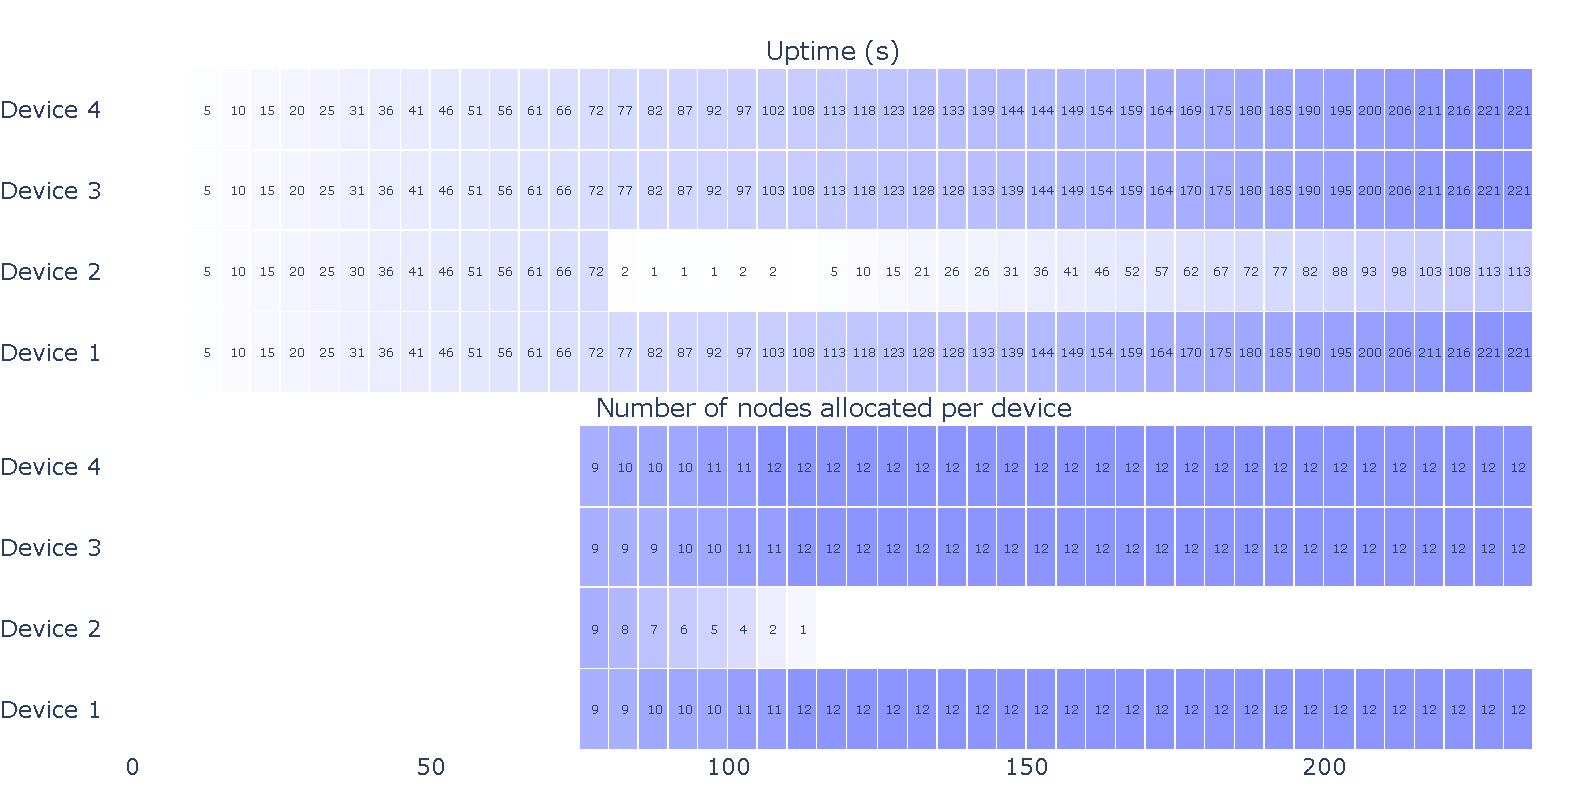
\includegraphics[width=\linewidth]{experiences/D-memory_error_random/memory_random.pdf}
\caption[Experiment D measurements]{Experiment D measurements}\label{fig:experiment_d_graph}
\end{figure}

%%%%%%%%%%%%%%%%%%%%%% Exp E %%%%%%%%%%%%%%%%%%%%%%

\subsubsection{Experiment E}

\textcolor{blue}{TODO}

This experiment purpose is inject a node that causes \textit{Out-of-Memory} errors in specific devices. With this, the system should (re)orchestrate and converge in a solution where the specific nodes are assigned to devices not affected by them. In their turn, the devices affected by these nodes should have less nodes assigned to them. The system and devices do not know that a specific node is creating the \textit{Out-of-Memory} errors and interpret the error as a device problem.

Since the first assignment can already be correct by default, meaning that these faulty nodes are assigned to devices not affected by them, some changes were made to force the system to (re)orchestrate. The devices were all turned off and on in in different order, this repeated 3 times. These events can be observed in Figure \ref{fig:experiment_e_graph} around the 125, 200 and 275 second timestamps.

\textcolor{red}{Acho que este gráfico não dá bem para perceber o que se está a passar. Já agora, esta experiência em si é uma repetição das duas outras. Isto é, testa o que as duas anteriores já testaram.}
\todo[inline]{Maybe remove this experiment. Graph can't convey what happens}

\begin{figure}[h]
\centering
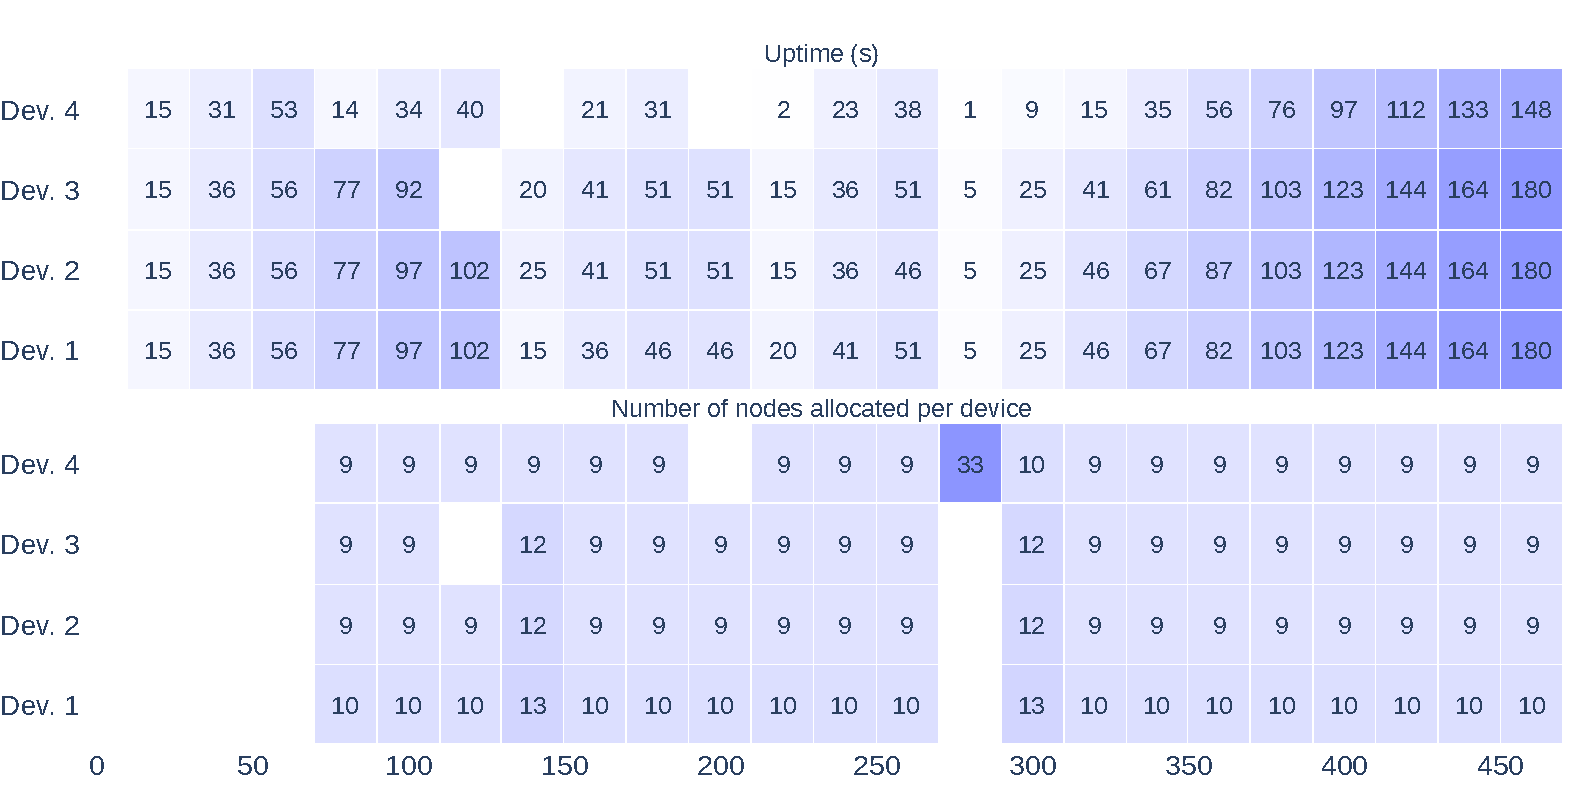
\includegraphics[width=\linewidth]{experiences/E-memory_error_node_failure/memory_failure.pdf}
\caption[Experiment E measurements]{Experiment E measurements}\label{fig:experiment_e_graph}
\end{figure}

%%%%%%%%%%%%%%%%%%%%%% Exp F %%%%%%%%%%%%%%%%%%%%%%

\subsubsection{Experiment F}

\textcolor{blue}{TODO}

\textcolor{red}{Possibly will have to repeat this experiment, since I can't find a pattern to note...its all a blob of events}

\begin{figure*}[h]
    \centering
    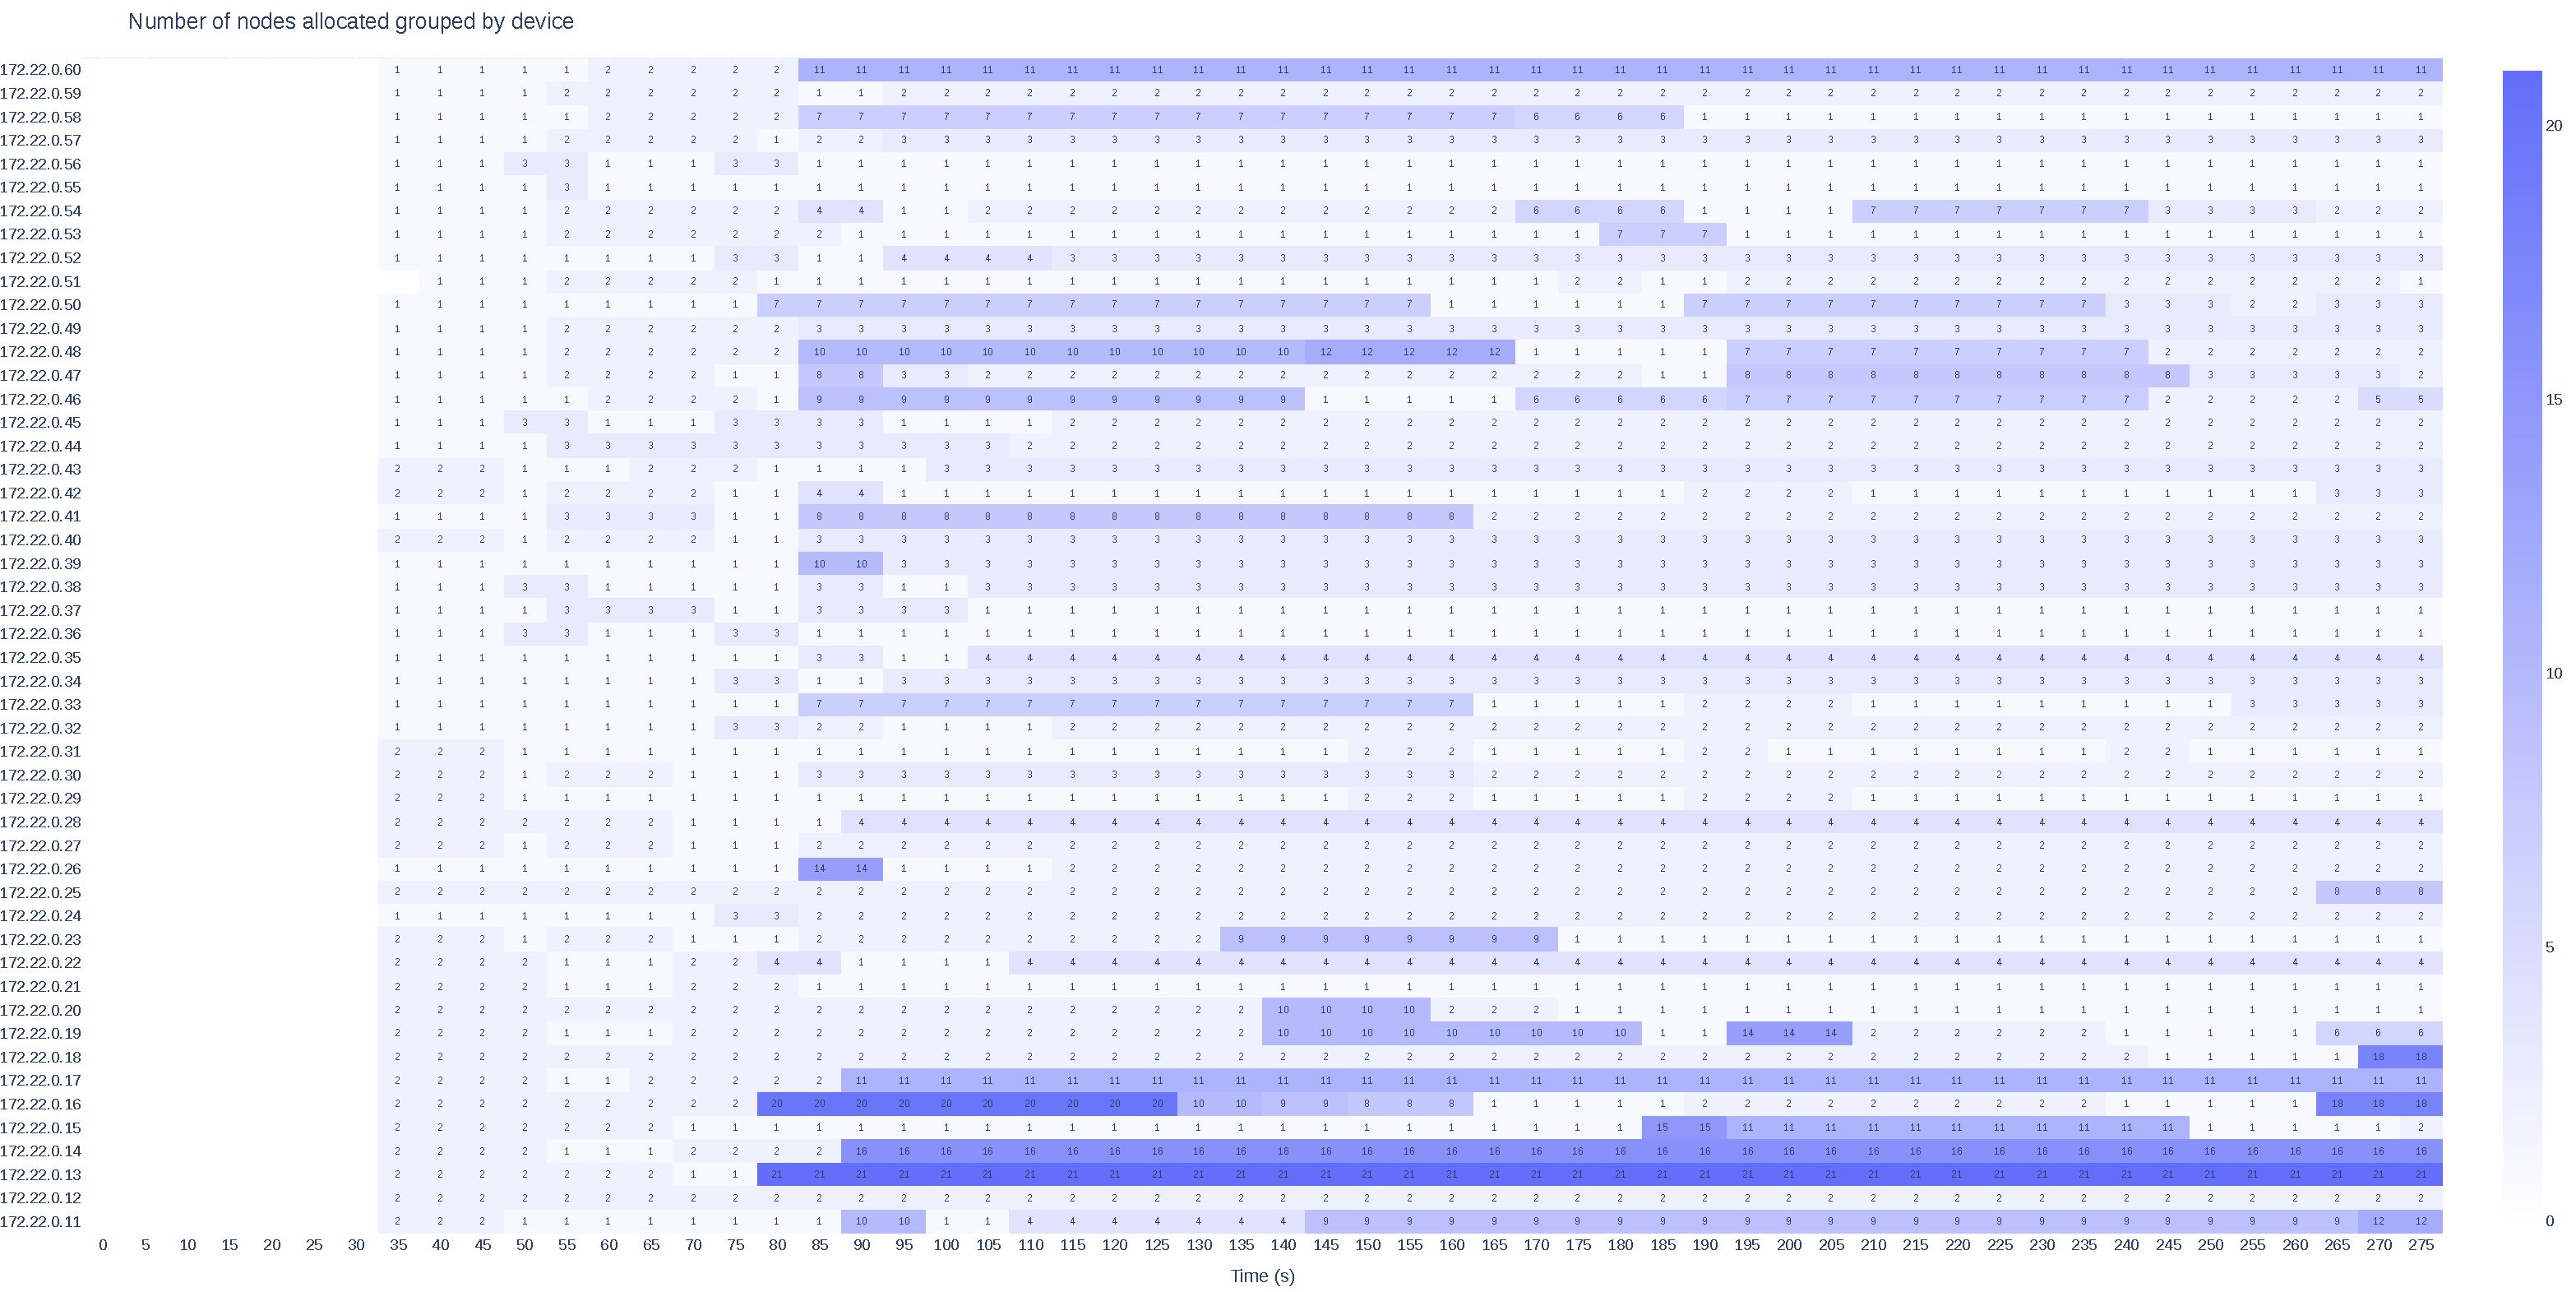
\includegraphics[width=\textwidth]{experiences/F-stress_test/nodes_heatmap.pdf}
    \caption[Nodes assignment distribution]{Nodes assignment distribution}\label{fig:stress_test_nodes}
\end{figure*}

\begin{figure}[h]
\centering
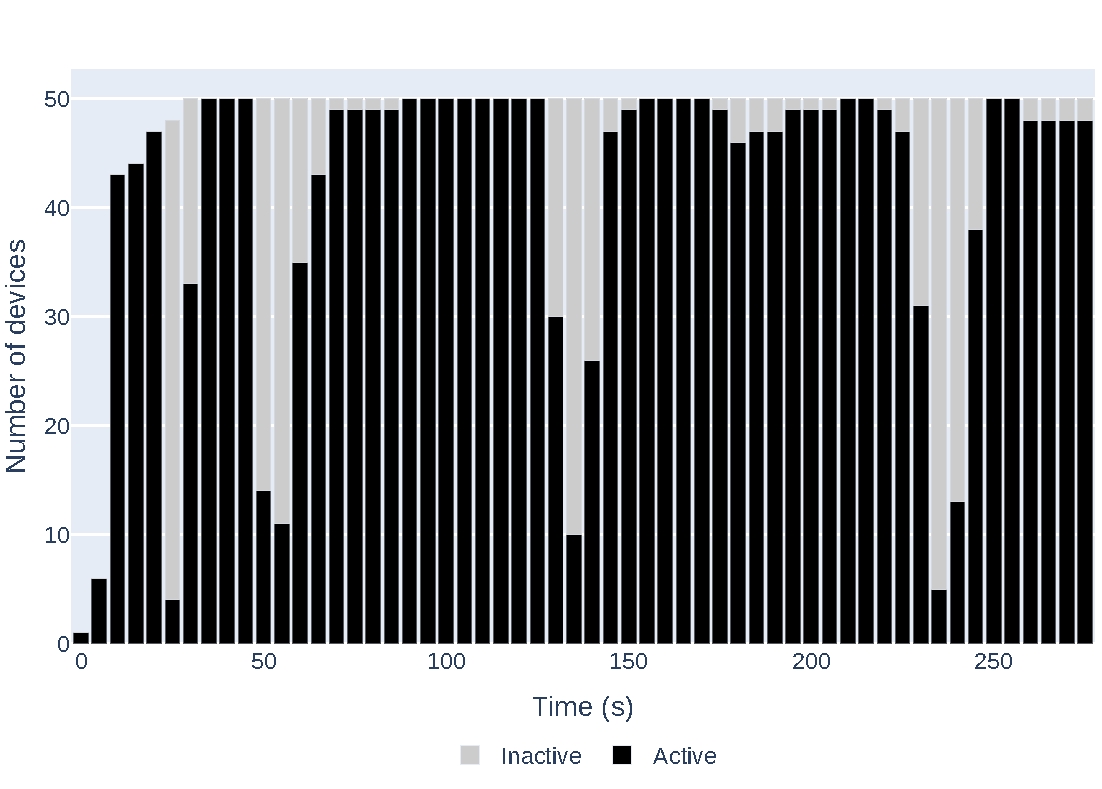
\includegraphics[width=\linewidth]{experiences/F-stress_test/status.pdf}
\caption[Number of devices active and inactive]{Number of devices active and inactive}\label{fig:stress_test_status}
\end{figure}

%%%%%%%%%%%%%%%%%%%%%%%%%%%%%%%%%%%%%%%%%%%%

\subsection{Scenario 2}\label{sec:discussion_scenario2}

As mentioned previously, several experiences were made to compare the developed solution to existing ones. To this end goal, a simple experiment of passing a message through several devices was implemented and the time the message takes to pass through all the devices was measured. The implementation of the scenario in the Node-RED tool is shown in Figure \ref{fig:scenario2_node_red}. The \textit{nothing} nodes execution consists of only redirecting their input to their output. The message consisting of the current timestamp is inserted into the system by the \textit{inject} node with user input, and the same message is showcased by the \textit{debug} node, the green one.

\begin{figure}[h]
\centering
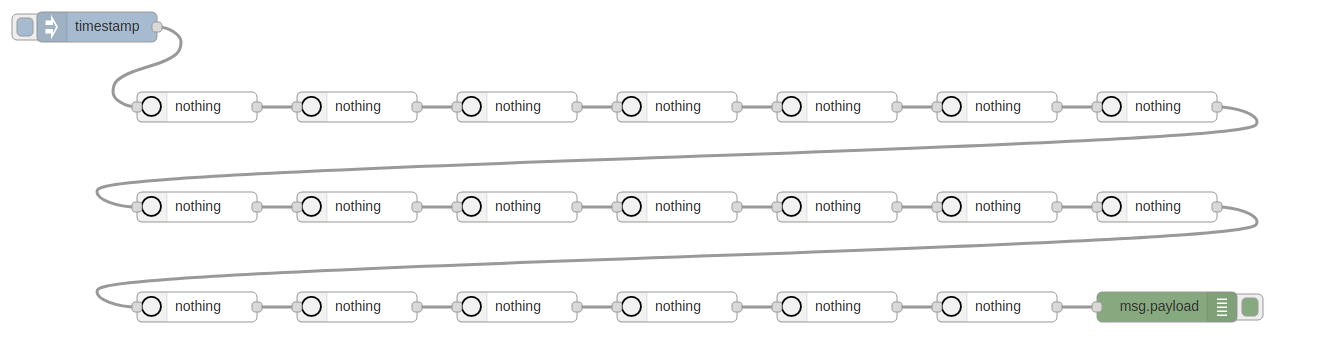
\includegraphics[width=\textwidth]{scenario2.png}
\caption[Node-RED implementation of scenario 2]{Node-RED implementation of scenario 2}\label{fig:scenario2_node_red}
\end{figure}

This same setup was replicated in several environments, as mentioned before. Each experiment was replicated 10 times, resulting in the data seen in the Appendix \ref{ap:scenario2_tables} tables. These tables were analysed to construct the Table \ref{tab:scenario2_table} and its visually representation in Figure \ref{fig:scenario2_candlestick}.

\captionsetup{belowskip=12pt,aboveskip=4pt}
\begin{table}[ht]
    \centering
    \resizebox{0.8\textwidth}{!}{%
    \begin{tabular}{ l  c  c  c  c }
        \toprule
        \textbf{Label} & \textbf{Min} & \textbf{Q2} & \textbf{Q3} & \textbf{Max}\\
        \midrule
        Node-RED original & 3 & 10 & 13.25 & 15 \\
        Node-RED + MQTT & 134 & 430.5 & 711.25 & 883 \\
        Node-RED modified + Dockers (same host) & 1217 & 1318 & 1573.75 & 1665 \\
        Node-RED modified + Dockers (different host) & 1445 & 2536 & 2708 & 3059 \\
        Physical + MQTT & 3616 & 4142 & 4372 & 4452 \\
        Node-RED modified + MQTT + Physical + Firmware & 4168 & 4569 & 5087.75 & 5940 \\
        \bottomrule
    \end{tabular}
    }
    \caption{Scenario 2 results}
    \label{tab:scenario2_table}
\end{table}{}

\begin{figure}[h]
\centering
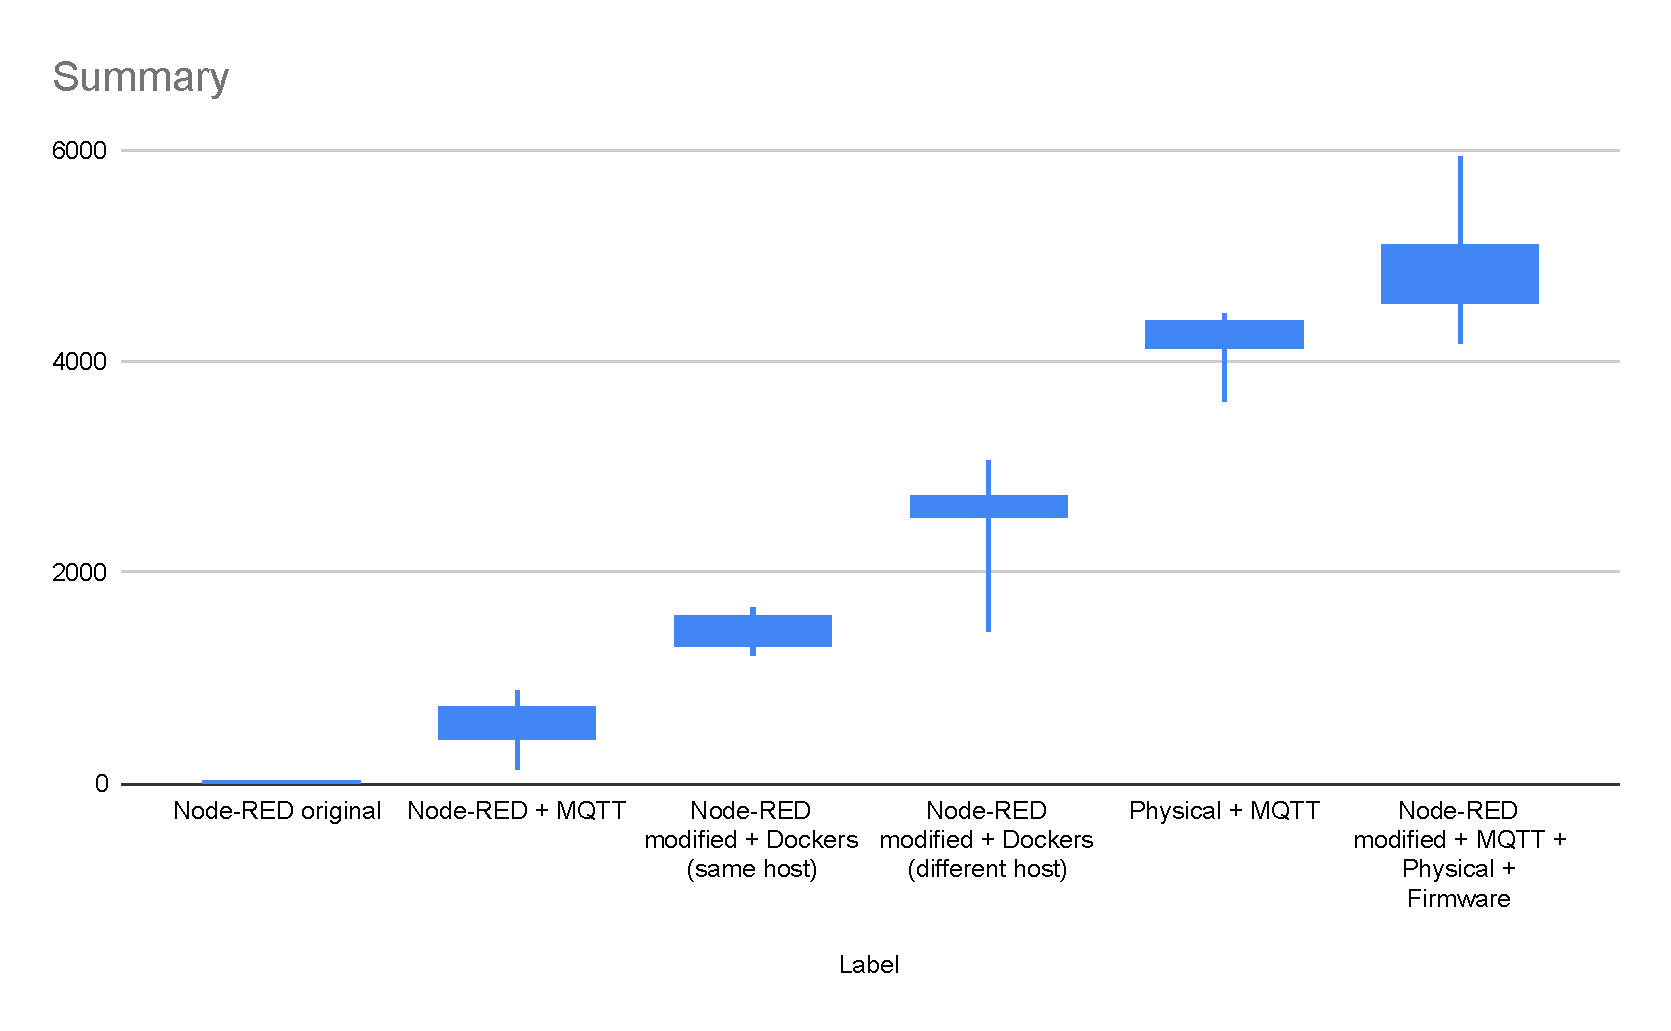
\includegraphics[width=\textwidth]{scenario2_graph.pdf}
\caption[Scenario 2 results]{Scenario 2 results}\label{fig:scenario2_candlestick}
\end{figure}

The Figure \ref{fig:scenario2_candlestick} demonstrates that the developed solution is considerably less efficient in communicating message between nodes. However, given the other experiences, it is possible to conclude that this lack of efficiency is caused not by the firmware created but because of the stack of communication the message as to go through, as well as the nature of MicroPython. 

When the decentralization is applied inside Node-RED, without running any MicroPython, it is possible to see that the introduction of a Mosquitto broker running in the same host causes some latency. The introduction of Dockers running the firmware in the same host as the Node-RED instance and Mosquitto broker causes more latency, making it possible to conclude that MicroPython of the developed firmware also delay de communication. By repeating the same experience as before but with the Mosquitto broker in another machine, it is noticeable that the times are more spread out and the overall latency of the system is bigger. Given the stacks of Wi-Fi that the message as to go through, this result is logical.

Lastly, the experiment was repeated in physical devices, first by running a simple code in he MicroPython flashed devices and insertion of the message using the Mosquitto client, and second by using the whole developed system, with the modified Node-RED and firmware in the devices. The results allows us to conclude that the devices produce the worst time, but firmware developed introduces little latency, visible by the comparison of both their results.

It is possible to conclude that the developed solution's node communication is slower than the original Node-RED mostly due to the nature of Wi-Fi communications and the MicroPython port used.   

\textcolor{red}{Add other tables with the timestamps in the annex}

\subsection{Overview}\label{sec:discussion_overview}

\textcolor{blue}{Overview of the evaluation of the system, with conclusions of the evaluation of the system as a whole}

\section{Conclusions}\label{sec:evaluation_conclusions}

